% For å referere til vedlegg bruk
%
% \ref{appendix:epost-skaar}
% \ref{appendix:intervju-skaar}
% \ref{appendix:plan-a}
%
% osv

%\documentclass{article}
%\usepackage{pdfpages}
%\usepackage{lipsum}
%\titleformat{\chapter}[hang]{\normalfont\huge\bfseries}{\chaptertitlename\ \thechapter}{10pt}{\huge}
%\titlespacing*{\chapter}
%  {0pt}{5pt}{5pt}
%Bruk chapter
%\section{Vedlegg}
%\chapter{Vedlegg}
%\tableofcontents
%\appendix

%PDF nr1
%\includepdf[pages=1, scale=.4, pagecommand={\chapter{Emailkorrespondanse -\\ Skanska v/John Skaar}\label{appendix:epost-skaar}}]{Vedlegg/Emailkorrespondanse-Skanska_v_John_Skaar.pdf}
%\includepdf[pages=2-, scale=0.6, pagecommand={\thispagestyle{plain}}]{Vedlegg/Emailkorrespondanse-Skanska_v_John_Skaar.pdf}
\setcounter{chapter}{0}
\renewcommand{\thechapter}{\Alph{chapter}}
\chapter{Microchip referance design form 1998}
\label{appendix:ASKreader}
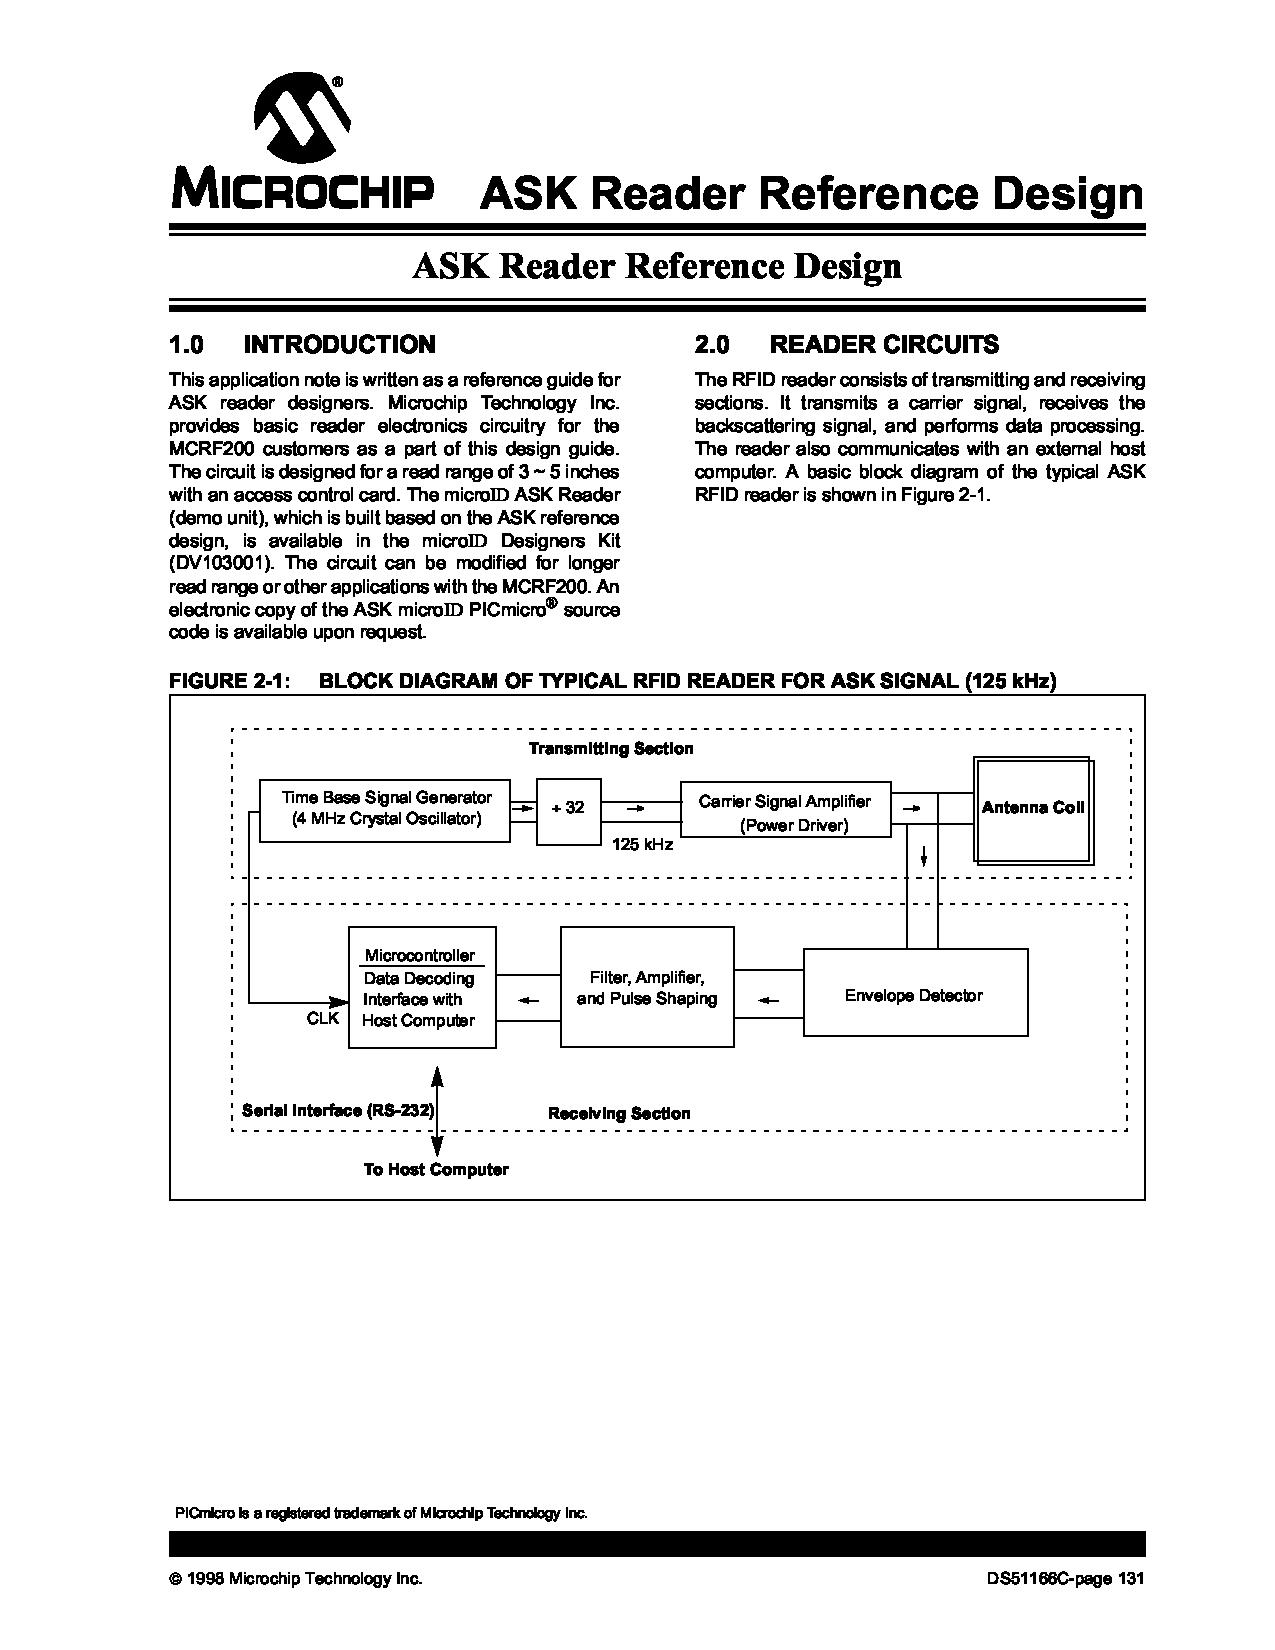
\includepdf[pages=1-6, scale=1]{Vedlegg/Appendix_125khz_microid.pdf}
\chapter{ATtiny 1617 RFID circuit}
\label{appendix:RFIDreader}
\begin{landscape}
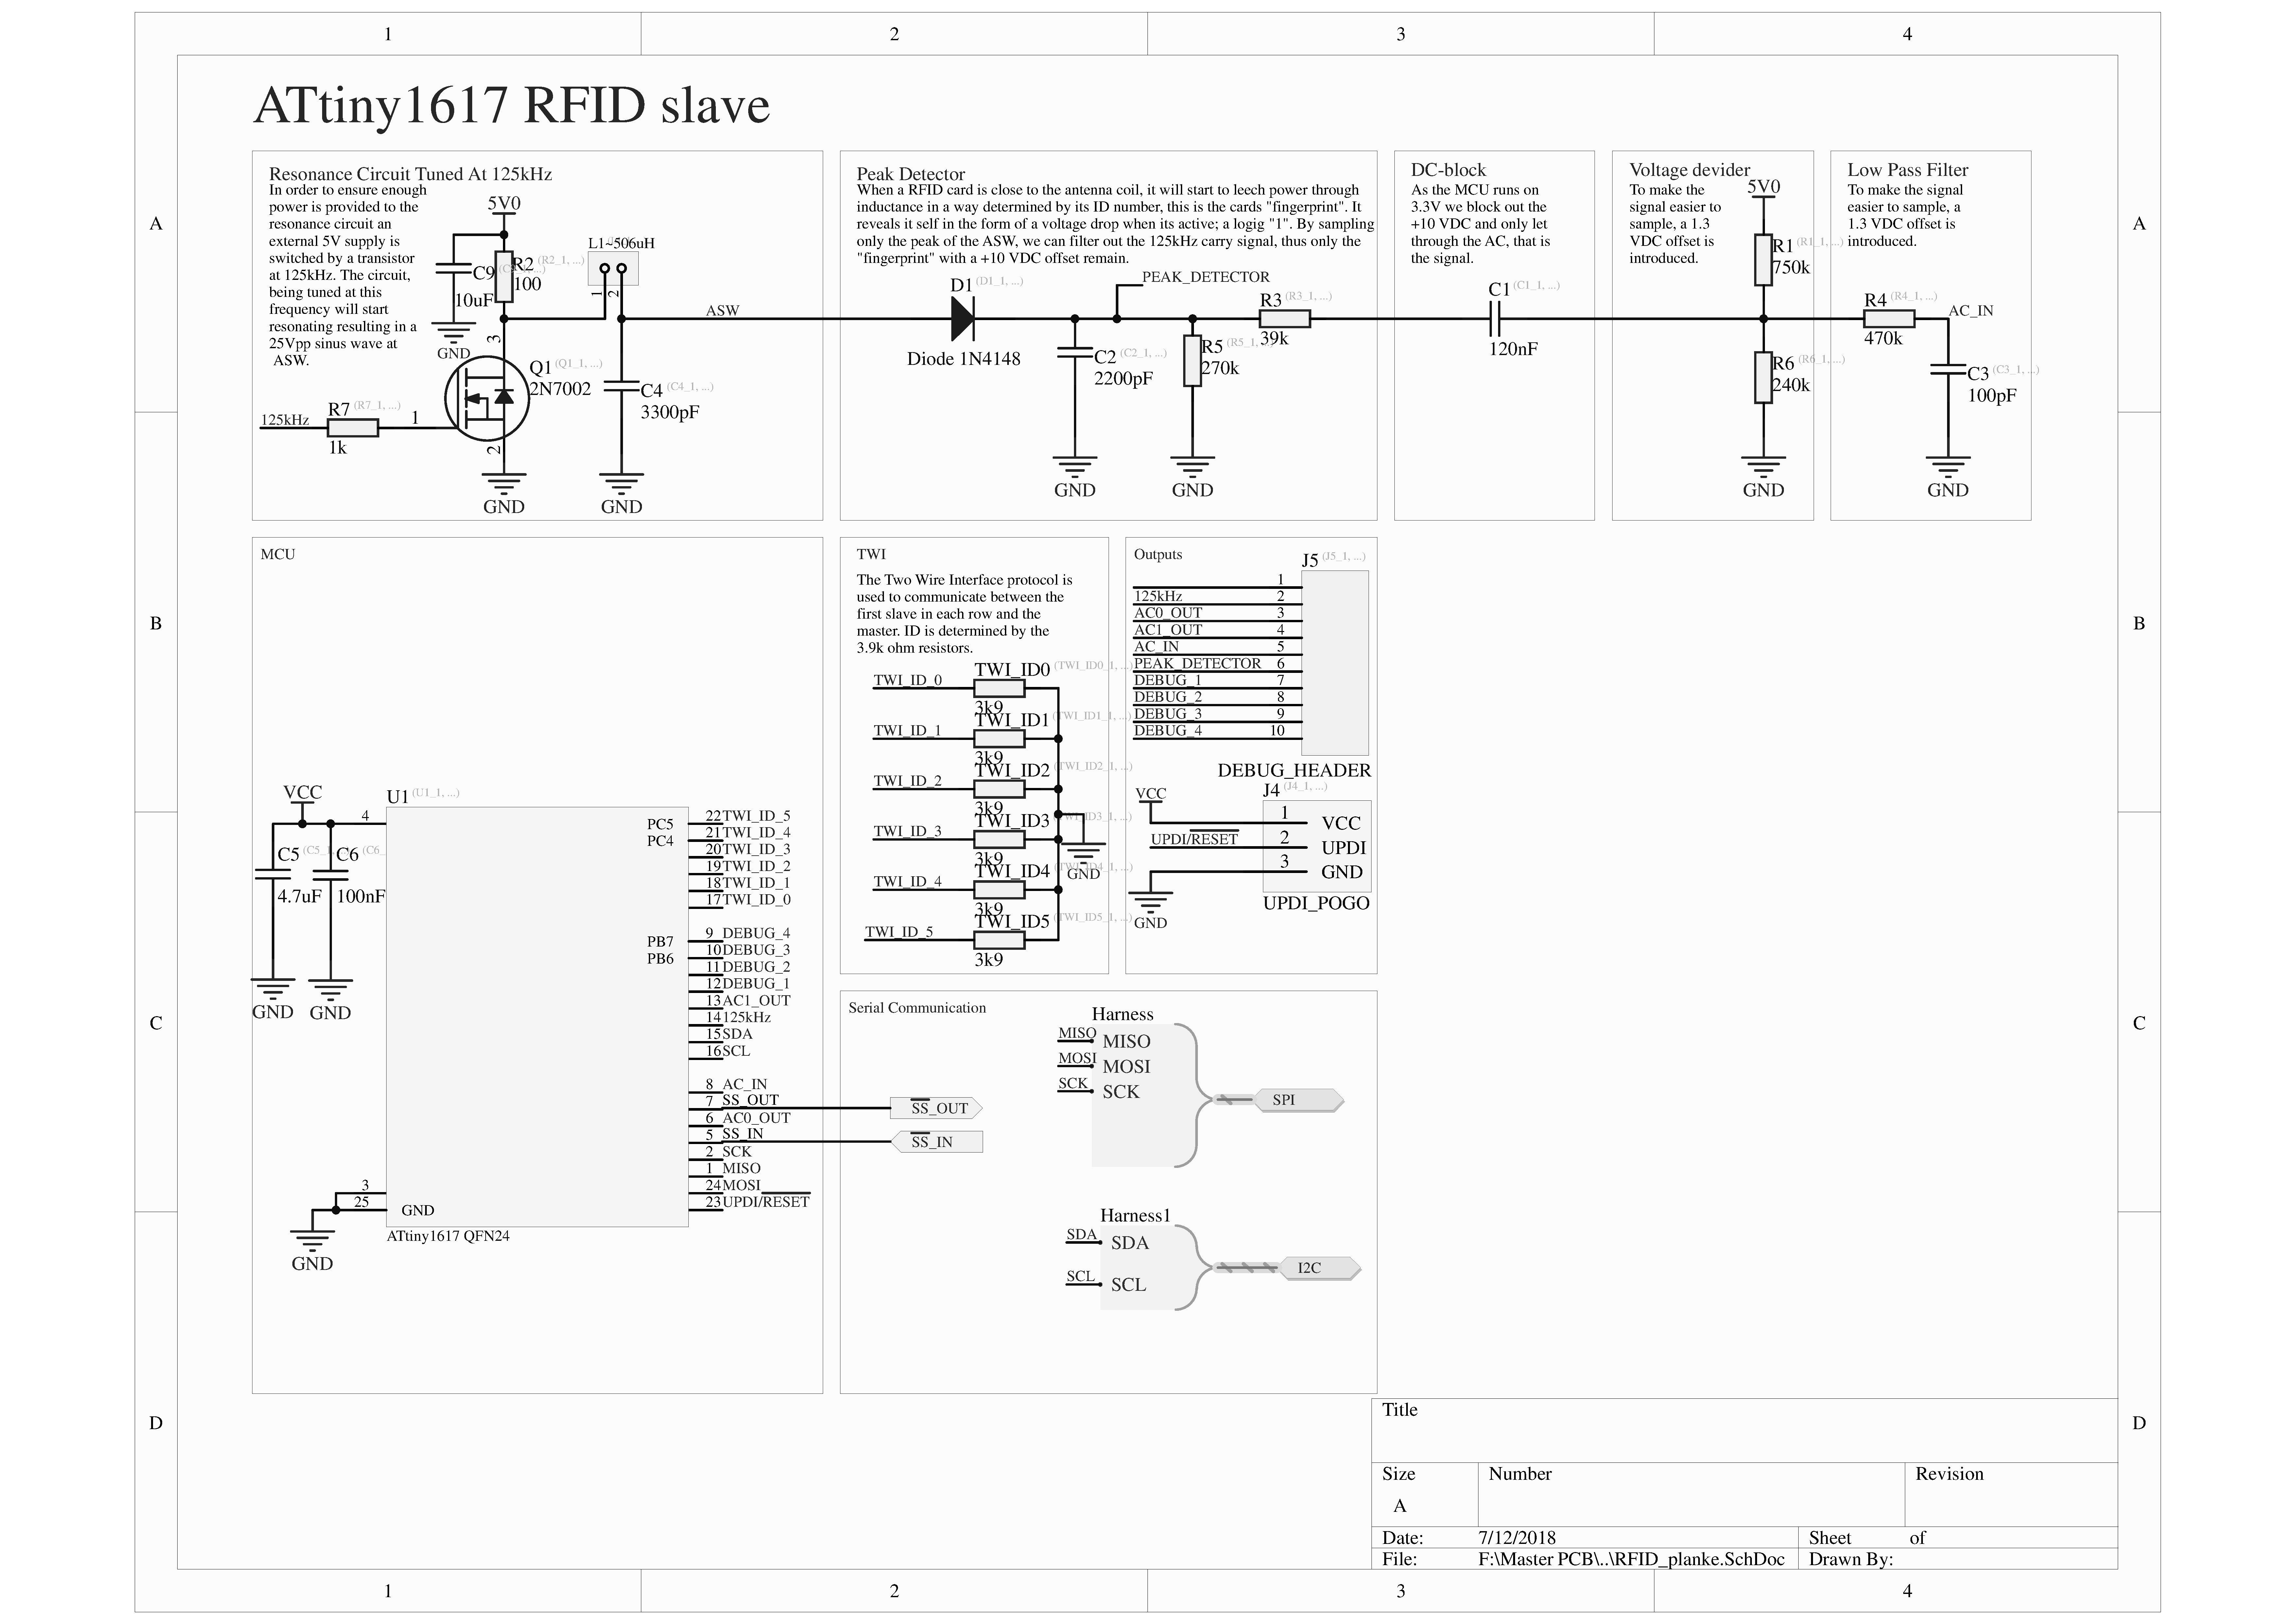
\includepdf[pages=1, scale=1,angle=90]{Vedlegg/RFID_circuit.pdf}
\end{landscape}

% PDF nrX osv nedover her
